\section{Ablation}\label{sec:ablation}

\subsection{Network start against early freeze}\label{sec:abl-four}

The candidate changed two things at once with respect to the published default: the start phases and the freeze index. Table~\ref{tab:ablation} separates them on the same $\nGeo$ geometries and seeds, and Figure~\ref{fig:ablation} shows the medians with their intervals and the share of runs that never reach 1 percent.
The early freeze alone, with no network, lowers the median from \itRTwelve{} to \itRThree{} iterations, a factor of \ratioRoverRThree{} (interval \ratioRoverRThreeLo{} to \ratioRoverRThreeHi), and the paired sign test over geometries rejects equality ($\signARRThree$ geometries need more iterations with the default, $\signBRRThree$ fewer, $\signTRRThree$ ties, $p=\signPRRThree$). The network alone, with the published freeze, does not change the median (\itNTwelve{} against \itRTwelve, factor \ratioRoverNTwelve{}; $\signARNTwelve$ against $\signBRNTwelve$ geometries, $p=\signPRNTwelve$). The combination of the two, the candidate, gives \itNThree{} iterations, a factor of
\ratioRoverN{}, which is below the factor of the early freeze alone (\ratioRoverRThree{}), and its sign test against the default has $p=\signPRN$, larger than that of the freeze alone. In every comparison the arm with the network is not better than the arm without it that has the same freeze index.

\begin{table}[t]
\centering\small
\resizebox{\textwidth}{!}{\begin{tabular}{@{}lccrrr@{}}
\toprule
Arm & Network start & Early freeze & Median it. & Ratio to the default [95\% CI] & Sign test $p$ \\
\midrule
engine default & no & no & 14 & 1 & -- \\
early freeze only & no & yes & 7.5 & 1.87 [1.38, 2.33] & 0.0032 \\
network only & yes & no & 14 & 1.00 [1.00, 1.00] & 0.29 \\
network and early freeze & yes & yes & 8 & 1.75 [0.85, 2.00] & 0.092 \\
\bottomrule
\end{tabular}
}
\caption{Ablation of the learned warm start on the $\nGeo$ held-out geometries: the network start and the early freeze index ($\nfix=3$ against the default 12) crossed, with the median iterations to 1\%, the ratio of the default's median to each arm's with a bootstrap 95\% interval, and the exact two-sided sign test against the default.}
\label{tab:ablation}
\end{table}

\begin{figure}[t]
\centering
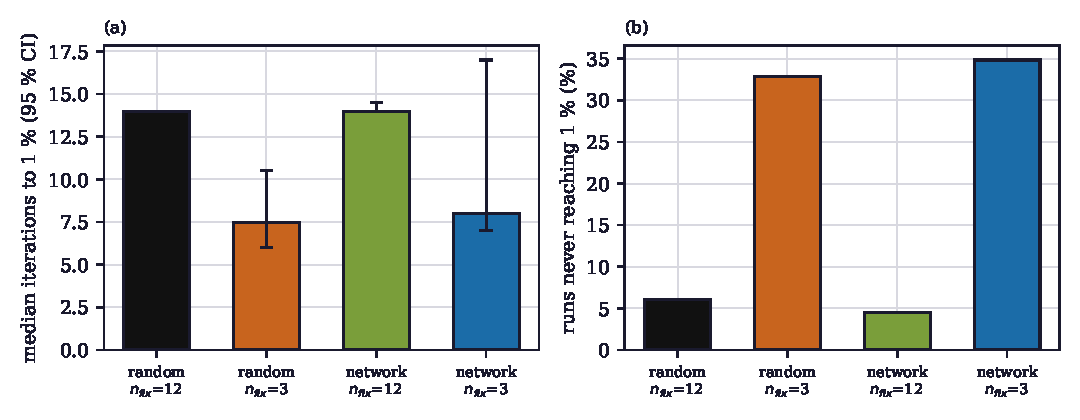
\includegraphics[width=\textwidth]{fig-ablation.pdf}
\caption{Ablation on the $\nGeo$ held-out geometries: (a) median iterations to 1\% with the bootstrap 95\% interval for the four arms; (b) share of the runs ($\nGeo$ geometries, $\nSeeds$ seeds) that do not reach 1\% within \budget{} iterations, which is the price of the early freeze whatever the start.}
\label{fig:ablation}
\end{figure}

The efficiency tells the same story. The final efficiency is \effmRTwelve{} at the default, \effmNTwelve{} for the network at $\nfix=12$ and \effmRThree{} and \effmNThree{} with the early freeze: the loss of efficiency that failed H2 is caused by the freeze (\effdRThree{} percent for a random start with it) and the network adds \effdNThreeRThree{} percent to it. The share of runs that never reach 1 percent shows what the early freeze buys the median with: \neverRThree{} percent for the random start at $\nfix=3$ and \neverNThree{} percent for the network, against \neverRTwelve{} and \neverNTwelve{} percent at the default.
A statistic that does not look at the tail, the median, hides that the early freeze fails to converge on about a third of the runs.

\subsection{Sweep of the freeze index}\label{sec:abl-sweep}

Table~\ref{tab:sweep} and Figure~\ref{fig:sweep} give the median iterations, the share that never converge and the final spread for the freeze index from $1$ to $12$, for both starts, on the $30$ geometries of the sweep. The median for the random start falls from \swTwelve{} iterations at $\nfix=12$ to \swEight{} at $8$, \swSix{} at $6$, \swFour{} at $4$ and \swThree{} at $3$, while the share of runs that never reach 1 percent rises from \swTwelveNever{} to \swEightNever{}, \swSixNever{}, \swFourNever{} and \swThreeNever{} percent. At $\nfix=2$ the median is the cap (the run does not converge on most geometries) and at $\nfix=1$ it is too:
\swOneNever{} percent of the runs never converge. The final spread rises as the freeze index falls, from \swTwelveFin{} percent at 12 to \swThreeFin{} at 3. The relation is a trade between iterations and the probability of reaching 1 percent, with a minimum of the median near $\nfix=4$.

The network start follows the random start along the whole sweep. At $\nfix=1$, where Proposition~\ref{prop:washout}(a) says the run is a function of the start phases alone and the network would have its fullest effect, the network start reaches 1 percent in the median in \swnOne{} iterations and fails to converge in \swnOneNever{} percent of the runs, against \swOneNever{} percent for the random start. At $\nfix=2$ the shares are \swnTwoNever{} and \swTwoNever{} percent, at $\nfix=3$ \swnThreeNever{} and \swThreeNever{}, at $\nfix=4$ \swnFourNever{} and \swFourNever{}, at $\nfix=6$ \swnSixNever{} and \swSixNever{} and at $\nfix=12$ \swnTwelveNever{} and \swTwelveNever{}. The medians differ by at most one iteration
wherever both are below the cap. The final spread of the network is lower than the random start's at several indices on this subset (at $\nfix=12$, \swnTwelveFin{} against \swTwelveFin{} percent), but it is higher over the full $\nGeo$ geometries (\finNTwelve{} against \finRTwelve{} percent), so the direction of the final-spread difference is not consistent and we do not claim one.

\begin{table}[t]
\centering\small
\resizebox{\textwidth}{!}{\begin{tabular}{@{}rrrrrrr@{}}
\toprule
$n_{\mathrm{fix}}$ & Random: median it. & Never (\%) & Final $\sigma$ (\%) & Network: median it. & Never (\%) & Final $\sigma$ (\%) \\
\midrule
1 & 61 & 76.7 & 34.3 & 61 & 80 & 52.2 \\
2 & 61 & 61.1 & 2.32 & 61 & 70 & 20.1 \\
3 & 9.5 & 41.1 & 0.512 & 10.5 & 40 & 0.213 \\
4 & 8 & 28.9 & 0.202 & 9 & 23.3 & 0.18 \\
6 & 10 & 14.4 & 0.0742 & 10 & 20 & 0.0371 \\
8 & 11 & 12.2 & 0.00997 & 12 & 16.7 & 0.0352 \\
12 & 14 & 7.8 & 0.00013 & 14 & 6.7 & 1.91e-05 \\
\bottomrule
\end{tabular}
}
\caption{Sweep of the freeze index $\nfix$ on 30 of the held-out geometries (every second generated geometry, $\nSeeds$ seeds): median iterations to 1\% (the value 61 means the median run does not reach 1\% within 60 iterations), share of runs that never reach it and median final spread, for a random start and for the network start.}
\label{tab:sweep}
\end{table}

\begin{figure}[t]
\centering
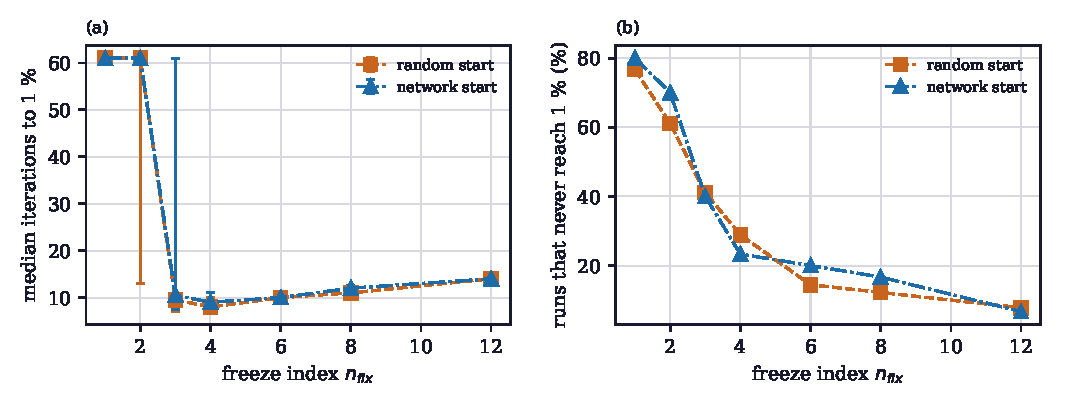
\includegraphics[width=\textwidth]{fig-sweep.pdf}
\caption{Sweep of the freeze index $\nfix$ on 30 held-out geometries for the random and the network start: (a) median iterations to 1\% with the bootstrap 95\% interval; (b) share of runs that never reach 1\% within \budget{} iterations. The two starts follow each other at every index.}
\label{fig:sweep}
\end{figure}

\subsection{Oracle start}\label{sec:abl-oracle}

The strongest start a predictor could be asked for is the converged solution of the iteration itself. Table~\ref{tab:oracle} and Figure~\ref{fig:oracle} give, for ten generated geometries and the first seed, the iterations to 1 percent from the phases of a converged random-start run. With the default freeze, the oracle start needs a median of \OTwelveMed{} iterations against \ORMed{} from the random start, a saving of \OTwelveGain{} iteration; at $\nfix=3$ it needs \OThreeMed{} against \ORThreeMed{}, and with the freeze at the first iteration \OOneMed{}. On the geometry that does not converge for
any arm (the largest array of the ten, \texttt{gen/06} in Table~\ref{tab:oracle}) the oracle does not help either. Two readings follow. First, at the published freeze index the start cannot be worth more than about one iteration, whoever predicts it: the network at $\nfix=12$ has nothing to improve. Second, with an oracle the early freeze converges on geometries on which the random start with the same freeze never does (\texttt{gen/01}, \texttt{gen/03} and \texttt{gen/08}), which is the part of the gap a perfect predictor could close; the network, with its phases, does not close it (Table~\ref{tab:sweep}). The predicted
phases are not those of a converged solution, which the trap list alone does not determine because the converged phases of a dense array depend on the random start that produced them.

\begin{table}[t]
\centering\small
\resizebox{\textwidth}{!}{\begin{tabular}{@{}lrrrrrr@{}}
\toprule
Held-out geometry & Traps & Random, 12 & Oracle, 12 & Random, 3 & Oracle, 3 & Oracle, 1 \\
\midrule
gen/00 & 236 & 13 & 11 & 7 & 5 & 5 \\
gen/01 & 345 & 18 & 14 & 61 & 8 & 8 \\
gen/02 & 448 & 14 & 13 & 16 & 6 & 6 \\
gen/03 & 456 & 15 & 13 & 61 & 7 & 6 \\
gen/04 & 133 & 14 & 13 & 7 & 5 & 5 \\
gen/05 & 102 & 13 & 13 & 5 & 5 & 4 \\
gen/06 & 768 & 61 & 61 & 61 & 61 & 61 \\
gen/07 & 679 & 13 & 8 & 4 & 4 & 4 \\
gen/08 & 450 & 16 & 14 & 61 & 9 & 8 \\
gen/09 & 140 & 5 & 2 & 4 & 2 & 2 \\
\bottomrule
\end{tabular}
}
\caption{Iterations to 1\% on ten held-out geometries (first seed) from a random start and from the oracle start (the phases of a converged random-start run) for freeze indices 12, 3 and 1; the value 61 means 1\% is not reached within 60 iterations.}
\label{tab:oracle}
\end{table}

\begin{figure}[t]
\centering
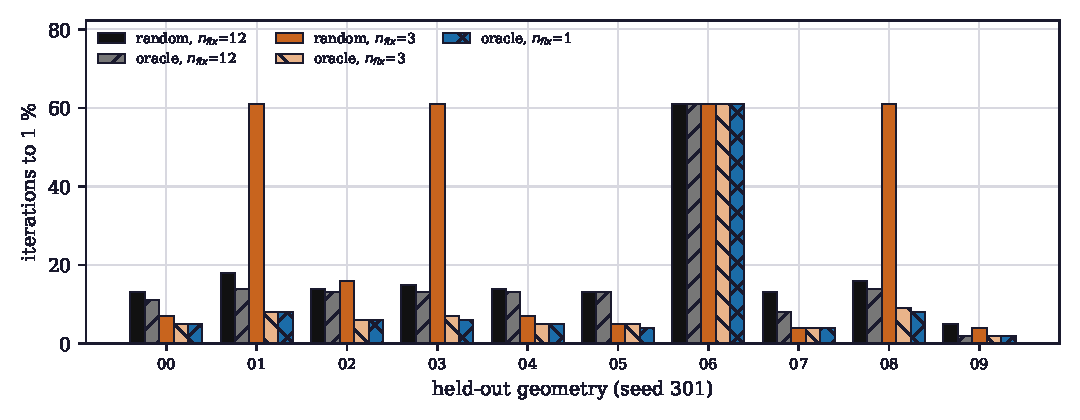
\includegraphics[width=\textwidth]{fig-oracle.pdf}
\caption{Iterations to 1\% on ten held-out geometries from a random start and from the oracle start for freeze indices 12, 3 and 1 (first seed); the bars at the top of the axis are runs that do not reach 1\% within the budget.}
\label{fig:oracle}
\end{figure}

\subsection{Weight accounting}\label{sec:abl-weights}

Table~\ref{tab:weights} and Figure~\ref{fig:weights} apply Proposition~\ref{prop:allowance} to the runs of the oracle comparison. The bound of Eq.~\eqref{eq:allowance} holds on all \wTwelveHold{} of \wTwelveN{} runs of each of the four conditions. It is loose: the weight spread of a converged run, a median of \wTwelveSMed{} for the random start at $\nfix=12$, is within reach of the allowance after a median of \wTwelveKMed{} iterations ($k_{\mathrm{floor}}$), while the median run needs \wTwelveItMed{} iterations to reach 1 percent. With an oracle start at $\nfix=12$ the corresponding numbers are \woTwelveKMed{} and
\woTwelveItMed{}. The restart of the weights at one therefore does not explain why 1 percent arrives at iteration 13 or later: the accounting identity permits the weights to rebuild their spread long before. This rules out the explanation that the weights, which restart, are the bottleneck, and it points to the freeze index as the quantity that sets the iteration count.

\begin{table}[t]
\centering\small
\resizebox{\textwidth}{!}{\begin{tabular}{@{}lrrrr@{}}
\toprule
Run (seed 301, ten geometries) & Median final $S$ & Median $k_{\mathrm{floor}}$ & Median it. to 1\% & Bound holds \\
\midrule
random start, $n_{\mathrm{fix}}=12$ & 0.71 & 2 & 14 & 10 of 10 \\
random start, $n_{\mathrm{fix}}=3$ & 1.43 & 3 & 11.5 & 10 of 10 \\
oracle start, $n_{\mathrm{fix}}=12$ & 0.67 & 4 & 13 & 10 of 10 \\
oracle start, $n_{\mathrm{fix}}=3$ & 0.80 & 5.5 & 5.5 & 10 of 10 \\
\bottomrule
\end{tabular}
}
\caption{Weight accounting on ten held-out geometries (first seed): median final log-spread $S$ of the weights, the first iteration $k_{\mathrm{floor}}$ at which the cumulative allowance of Eq.~\eqref{eq:allowance} reaches that spread, the median iterations to 1\%, and the number of runs on which the bound holds, for the random and the oracle start at two freeze indices.}
\label{tab:weights}
\end{table}

\begin{figure}[t]
\centering
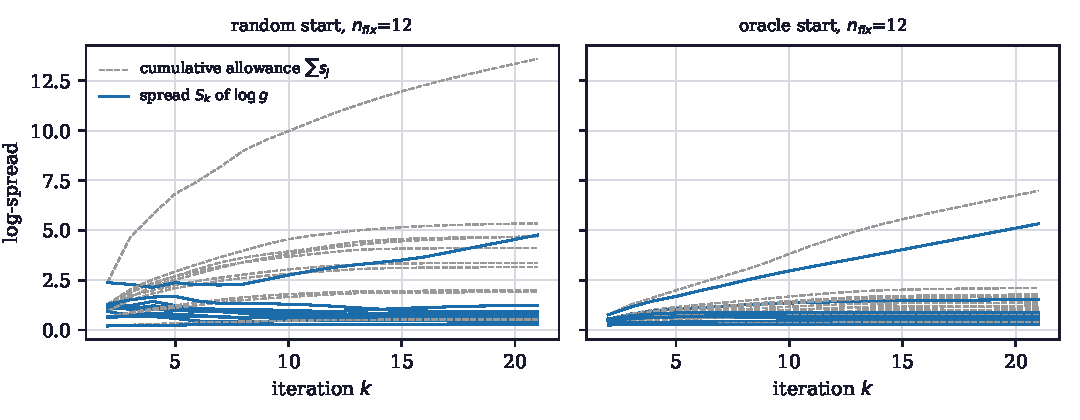
\includegraphics[width=\textwidth]{fig-weights.pdf}
\caption{Log-spread $S_k$ of the weights after iteration $k$ (solid) and the cumulative allowance $\sum_{j\le k}s_j$ of Eq.~\eqref{eq:allowance} (dashed), for ten held-out geometries at $\nfix=12$, from the random start (left) and the oracle start (right); the solid curves stay below the dashed ones on every run.}
\label{fig:weights}
\end{figure}
